\documentclass[a4paper,11pt,titlepage]{article}
% The maths package
\usepackage{amsmath}
% The graphics package
\usepackage{graphicx}
% Allows paragraph in blocks
\usepackage{parskip}
% Code hightling
\usepackage{minted}
% Verbatim file inclusion
\usepackage{fancyvrb}

%%%%%%%%%%%%%%%%%%%%%%%%%%%%%%%% Define the title %%%%%%%%%%%%%%%%%%%%%%%%%%%%%%
\title{
MECH3750 Engineering Analysis II \\ 
Assignment 1: Buckling analysis
}
% define the author
\author{
Merrick Heley\\
42339915
\and
Sophia Impiccini\\
42650852
}

%%%%%%%%%%%%%%%%%%%%%%%%%% Notes, commands, settings %%%%%%%%%%%%%%%%%%%%%%%%%%%
% \section*{Task 1} uses an asterisk to suppress the section number

% This command adds \ud for finishing integrals
\newcommand{\ud}{\,\mathrm{d}}

% Set the pygmentation style for code
% pygmentize -L styles
\usemintedstyle{autumn}

% Simple command for python file input
\newcommand{\inputpython}[1]{
    \inputminted[linenos=true, 
                 frame=single, 
                 fontsize=\scriptsize, 
                 label=#1]
                {python}{#1}
}

% Simple command for python file output
\newcommand{\pythonoutput}[1]{
    \immediate\write18{python #1 > #1.out}
    \fvset{frame=single, numbers=left, fontsize=\scriptsize, label=#1.out}
    \VerbatimInput{#1.out}
    \write18{del #1.out}
}

%%%%%%%%%%%%%%%%%%%%%%%%%%%%%%%% Start document %%%%%%%%%%%%%%%%%%%%%%%%%%%%%%%%

\begin{document}
% generates the title
\maketitle

%%%%%%%%%%%%%%%%%%%%%%%%%%%%%%%%%% TASK 1 %%%%%%%%%%%%%%%%%%%%%%%%%%%%%%%%%%%%%%
\section*{Task 1}

The Euler load is the load where the spring initially begins to bend.

\begin{figure}[!hbp]
\centering
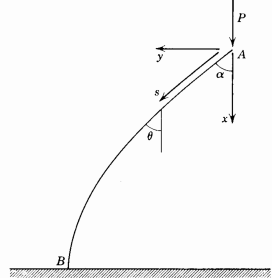
\includegraphics{buckling.png}
\caption{Buckling example}
\end{figure}

Where P is the load at A, $\theta$ is the angle of the bend at distance s 
from A.

For a rod placed vertically and fixed at end B, it can be seen that the initial
value of $\alpha$ is 0$^\circ$.

Using the given equation

\begin{equation}
L = 
\sqrt{\frac{EI}{P}} 
\int_0^{\frac{\pi}{2}} 
    {\displaystyle{\left[
        1-\sin^2{\left(\frac{\alpha}{2}\right)}\sin^2{\phi}
    \right]^{-\frac{-}{2}}}}
\ud \phi \label{eq:L}
\end{equation}

and substituting in the observation that the Euler load will be applied when the
rod is vertical

\begin{equation}
\alpha = 0 \text{ when } P = P_e
\end{equation}
the equation can be simplified 

\begin{align}
L & = 
\sqrt{\frac{EI}{P_e}} 
\int_0^{\frac{\pi}{2}} 
    {\displaystyle{\left[
        1-\sin^2{\left(\frac{0}{2}\right)}\sin^2{\phi}
    \right]^{-\frac{1}{2}}}}
\ud \phi \notag\\
& = 
\sqrt{\frac{EI}{P_e}} 
\int_0^{\frac{\pi}{2}} 
    {\displaystyle{\left[
        1-\sin^2{0}\sin^2{\phi}
    \right]^{-\frac{1}{2}}}}
\ud \phi \notag\\
& = 
\sqrt{\frac{EI}{P_e}} 
\int_0^{\frac{\pi}{2}} 
    {\displaystyle{\left[
        1
    \right]^{-\frac{1}{2}}}}
\ud \phi \notag\\
& = 
\sqrt{\frac{EI}{P_e}} 
\int_0^{\frac{\pi}{2}} \ud \phi \notag\\
& = \sqrt{\frac{EI}{P_e}} \left(\frac{\pi}{2} - 0\right) \notag\\
& = \frac{\pi}{2} \sqrt{\frac{EI}{P_e}} \notag\\
\intertext{and rearranged for $P_e$} \notag\\
\frac{2L}{\pi} & = \sqrt{\frac{EI}{P_e}} \notag\\ 
\frac{4L^2}{\pi^2} & = \frac{EI}{P_e} \notag\\
P_e & = \frac{\pi^2 EI}{4L^2} \label{eq:Pe}
\end{align}
\clearpage

%%%%%%%%%%%%%%%%%%%%%%%%%%%%%%%%%% TASK 2 %%%%%%%%%%%%%%%%%%%%%%%%%%%%%%%%%%%%%%
\section*{Task 2}
The code below implements an adaptive integrator that may take Gaussian
quadrature functions as input.

The ouput of the adaptive integrator test is provided, showing how closely the
integrator matches the SciPy integrator.
\\
\inputpython{integrator.py}
\pythonoutput{integrator.py}

It can be seen from the output that the adaptive integrator is quite accurate
compared to the module provided by SciPy.
\clearpage

%%%%%%%%%%%%%%%%%%%%%%%%%%%%%%%%%% TASK 3 %%%%%%%%%%%%%%%%%%%%%%%%%%%%%%%%%%%%%%
\section*{Task 3}

To compute the value of $\alpha$ given $\frac{x_g}{L}$, an expression for $x_g$
must be found (as an equation for L already exists in 
\eqref{eq:L}).
\begin{align}
\intertext{It can be noted that if}
\frac{\ud y}{\ud s} & = \sin{\theta} \label{eg:dyds}
\intertext{Then}
\frac{\ud x}{\ud s} & = \cos{\theta} \label{eq:dxds}
\intertext{Using the given equation}
\frac{\ud s}{\ud \theta} & = -\left [ \left(\frac{2P}{EI}\right)
			(\cos{\theta}- \cos{\alpha}) \right ]^{-\frac{1}{2}} \label{eq:dsdt}
\intertext{Chain rule can be used to cancel d$s$ by multiplying 
            \eqref{eq:dxds} and \eqref{eq:dsdt}}
\frac{\ud x} {\ud s} \cdot \frac{\ud s} {\ud \theta} & = 
			- \cos{\theta} \left [\left (\frac {2P}{EI}\right ) (\cos{\theta}- 
					\cos{\alpha}) \right ]^{-\frac{1}{2}} \notag\\
\frac{\ud x} {\ud \theta} & = 
			- \cos{\theta} \left [\left (\frac {2P}{EI}\right ) (\cos{\theta}- 
					\cos{\alpha}) \right ]^{-\frac{1}{2}} \notag\\
\intertext{As the region of interest is between point A and point B, the 
            integral should be over the region $x=0$ to $x=x_g$ where 
            $\theta = 0$ at $x=0$ and where $\theta = \alpha$ at $x=x_g$  }
\int_{0}^{x_g} \ud x & = \int_{0}^{\alpha} - \cos{\theta} \left [ \left(
			\frac{2P}{EI} \right )\left (\cos{\theta} - \cos{\alpha} \right )
					\right ]^{-\frac{1}{2}} \ud \theta \notag\\
x_g & = \int_{0}^{\alpha} - \cos{\theta} \left [ \left(\frac{2P}{EI} \right )
			\left (\cos{\theta} - \cos{\alpha} \right )\right ]^{-\frac{1}{2}} 
			\ud \theta \label{eq:xg}
\intertext{Dividing \eqref{eq:xg} by \eqref{eq:L} and simplifying gives}
\frac{x_g}{L} & = \frac {\int_{0}^{\alpha} - \cos{\theta} \left [ \left
(\frac{2P}{EI} \right)\left (\cos{\theta} - \cos{\alpha} \right )
\right ]^{-\frac{1}{2}}}{\sqrt {\frac {EI}{P}} \int_{0}^{\frac{\pi}{2}}\left[1 
- \sin^2\left({\frac {\alpha}{2}} \right )\sin^2 {\phi} \right]^{- \frac{1}{2}}
\partial \theta} \notag\\
& = \frac {\frac {1}{\frac {2P}{EI}} \int_{\alpha}^{0} -\cos{\theta}(\
cos{\theta} - \cos{\alpha})^{- \frac{1}{2}}\: \partial \theta} {{\frac {EI}{P}}
 \int_{0}^{\frac{\pi}{2}}\left[1 - \sin^2\left({\frac {\alpha}{2}} \right )
 \sin^2 {\phi} \right]^{- \frac{1}{2}}\partial \theta} \notag\\
 & = \frac {1}{\sqrt{2}} \frac {\int_{\alpha}^{0} -\cos{\theta}(\cos{\theta}
 - \cos{\alpha})^{- \frac{1}{2}}\: \partial \theta} {\int_{0}^{\frac{\pi}{2}}
 \left[1 - \sin^2\left({\frac {\alpha}{2}} \right ) \sin^2 {\phi} \right]^{- 
 \frac{1}{2}}\partial \theta} \label{eq:xgonl}
\intertext{To find a similar equation for $\frac{y_b}{L}$, the same process can
            be followed but the chain rule should be applied to \eqref{eg:dyds}
            and \eqref{eq:dsdt}}
\frac{y_b}{L} 
 & = \frac {1}{\sqrt{2}} \frac {\int_{\alpha}^{0} -\sin{\theta}(\cos{\theta}
 - \cos{\alpha})^{- \frac{1}{2}}\: \partial \theta} {\int_{0}^{\frac{\pi}{2}}
 \left[1 - \sin^2\left({\frac {\alpha}{2}} \right ) \sin^2 {\phi} \right]^{- 
 \frac{1}{2}}\partial \theta} \label{eq:xgonl}
\intertext{And an equation for $\frac{P}{P_e}$ can be found by first finding an
            equation for P by rearranging \eqref{eq:L}}
L &= \sqrt{\frac{EI}{P}} \int_0^{\frac{\pi}{2}} {\displaystyle{\left[
        1-\sin^2{\left(\frac{\alpha}{2}\right)}\sin^2{\phi}
    \right]^{-\frac{1}{2}}}} \ud \phi \notag\\
L^2 &= \frac{EI}{P} \left(\int_0^{\frac{\pi}{2}} {\displaystyle{\left[
        1-\sin^2{\left(\frac{\alpha}{2}\right)}\sin^2{\phi}
    \right]^{-\frac{1}{2}}}} \ud \phi \right)^2 \notag\\
P &= \frac{EI}{L^2} \left(\int_0^{\frac{\pi}{2}} {\displaystyle{\left[
        1-\sin^2{\left(\frac{\alpha}{2}\right)}\sin^2{\phi}
    \right]^{-\frac{1}{2}}}} \ud \phi \right)^2 \label{eq:P}
\intertext{and dividing \eqref{eq:P} by \eqref{eq:Pe} and simplifying.}
\frac{P}{P_e} &=
 \frac{\frac{EI}{L^2} \left(\int_0^{\frac{\pi}{2}} {\displaystyle{\left[
        1-\sin^2{\left(\frac{\alpha}{2}\right)}\sin^2{\phi}
    \right]^{-\frac{1}{2}}}} \ud \phi \right)^2}
      {\frac{\pi^2 EI}{4L^2}} \notag\\
 &= \frac{\left(\int_0^{\frac{\pi}{2}} {\displaystyle{\left[
        1-\sin^2{\left(\frac{\alpha}{2}\right)}\sin^2{\phi}
    \right]^{-\frac{1}{2}}}} \ud \phi \right)^2}
      {\frac{\pi^2}{4}} \notag\\
 &= \frac{4}{\pi^2} \left(\int_0^{\frac{\pi}{2}} {\displaystyle{\left[
        1-\sin^2{\left(\frac{\alpha}{2}\right)}\sin^2{\phi}
    \right]^{-\frac{1}{2}}}} \ud \phi \right)^2
\end{align}

As there are 3 equations and 4 unknowns, a value must be given in order to make
the equations solvable. The value given in this case was $\frac{x_g}{L}$.

\eqref{eq:xgonl} contains $\frac{x_g}{L}$ and a single other variable, but also
 contains an  elliptic integral which is not algebraically solvable. Numerical 
 methods must therefore be applied to resolve $\alpha$ if a value of 
 $\frac{x_g}{L}$ is known. The equation must first be put in the correct format 
 for optimisation:

\begin{equation}
 f\left(\alpha, \frac{x_g}{L}\right) 
  = \frac {1}{\sqrt{2}} \frac {\int_{\alpha}^{0} -\cos{\theta}(\cos{\theta}
 - \cos{\alpha})^{- \frac{1}{2}}\: \partial \theta} {\int_{0}^{\frac{\pi}{2}}
 \left[1 - \sin^2\left({\frac {\alpha}{2}} \right ) \sin^2 {\phi} \right]^{- 
 \frac{1}{2}}\partial \theta} - \frac{x_g}{L} \label{eq:fa}
\end{equation}

Now the equation is in the correct form, the equation can be solved for alpha 
using the bisection method and the values of $\frac{x_g}{L}$ 
(0.99, 0.95, 0.9, 0.5). To prevent calculating over discontinuous regions, 
the limits of the bisection 
method were set to be between 0.01 and 0.99$\pi$ instead of 0 to $\pi$ for 
$\alpha$.
\clearpage

The values of 4 variables are shown below, where $\frac{x_g}{L}$ is the control
variable. The code is provided on the following page, and the appendix contains
the code used for the bisection method.
\\
% Get the output of task3.py
\immediate\write18{python task3.py > task3.py.out}

% Display the syntax and output of task3
\fvset{frame=single, numbers=left, fontsize=\scriptsize, label=task3.py.out}
\VerbatimInput{task3.py.out}
\write18{del task3.py.out}

\begin{figure}[!hbp]
\centering
\includegraphics[scale=0.6]{graph.png}
\caption{Graph generated by Task3}
\end{figure}

\clearpage
\inputpython{task3.py}
\clearpage

%%%%%%%%%%%%%%%%%%%%%%%%%%%%%%%% APPENDICES %%%%%%%%%%%%%%%%%%%%%%%%%%%%%%%%%%%%
\section*{Appendix A}
% Bisection method in appendix (shitty, and not correct way of doing appendices)
\inputpython{mybisect.py}
\pythonoutput{mybisect.py}



\clearpage
\end{document}